\documentclass[11pt]{jarticle}

\usepackage[dvipdfmx]{graphicx}
\usepackage{listings}
\usepackage{url}

\lstset{
    basicstyle={\ttfamily\small}, %書体の指定
    frame=tRBl, %フレームの指定
    framesep=10pt, %フレームと中身(コード)の間隔
    breaklines=true, %行が長くなった場合の改行
    linewidth=16cm, %フレームの横幅
    lineskip=-0.5ex, %行間の調整
    tabsize=2 %Tabを何文字幅にするかの指定
}

\setlength{\oddsidemargin}{-6.35mm}
\setlength{\textwidth}{171.9mm}

\begin{document}

\title{画像処理実験 第6回}
\author{09430565\\大橋虎ノ介}
\date{\number\year 年\number\month 月\number\day 日}
\maketitle

\section{概要}

 今回の実験では,各画像から得られた特徴点群の対応付けを行う処理を記述する.
各画像の特徴点群のすべての組み合わせに対して,類似度を計算しこの中から同一
物体を指す組を見つける.

使用する類似度の指標は,特徴点周辺の小領域の画素地の差の2乗和である.

\section{類似度の表を完成させる}

第1画像の第i特徴点と第2画像の第j特徴点の類似度をすべての組について計算し,
行列(i, j)に格納した表を作成する.

特徴点周辺の小領域の画素地の差の2乗和は以下のように計算される.
ここで,T1[i],T2[j]はi,j番目の特徴点周辺15x15の画素値を並べたベクトルを指す.

\[ SSD(i,j) = | T1[i] - T[j] |^{2} \]

以下の画像(0.jpg, 1.jpg)を入力し,それぞれの画像に対する特徴点群を便宜的に以下のように
設定した.

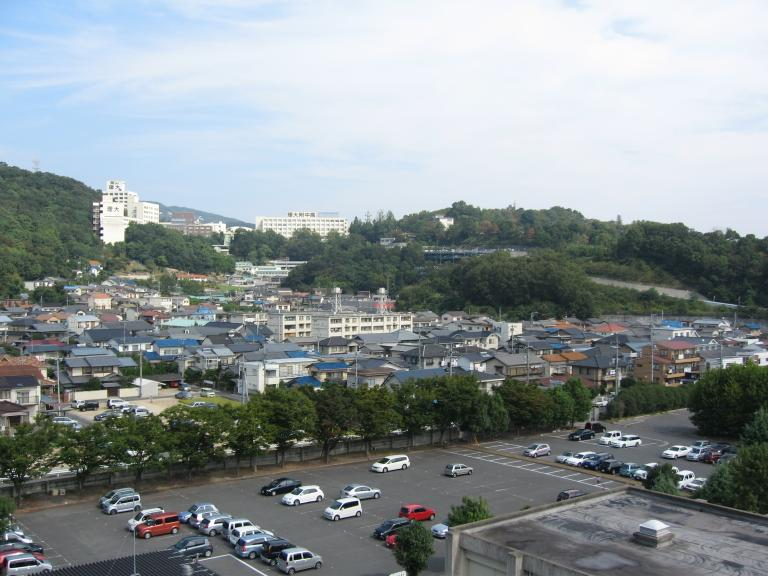
\includegraphics[scale=.3]{./img/0.jpg}
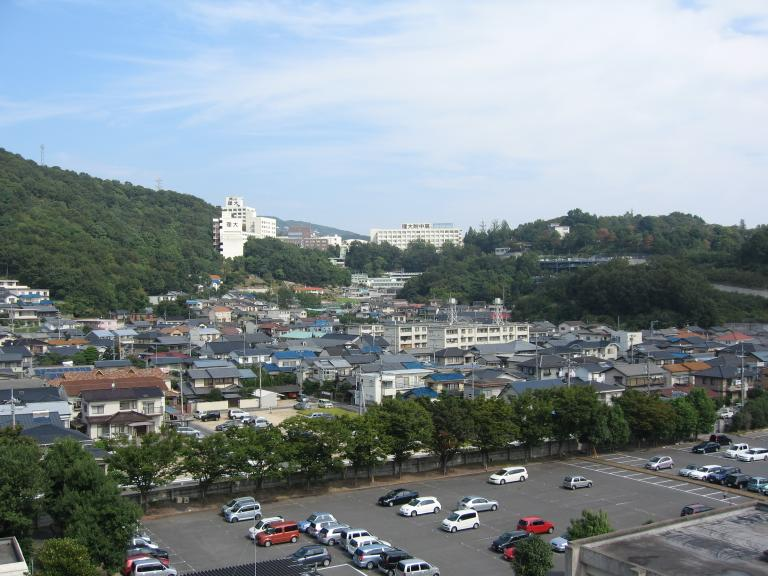
\includegraphics[scale=.3]{./img/1.jpg}

0.jpg:(234,456)(123,456)

1.jpg:(334,456)(223,456)

その結果,得られた類似度の表を以下に示す.

\[
  \left(
    \begin{array}{cc}
      3332651 & 1997656 \\
      2546873 & 1318164 
    \end{array}
  \right)
\]

\section{自動対応付けの方法}

前章で得られる類似度の表から,同一物体を指す特徴点を選ぶ.
その時,次の3つの条件を満たす必要がある.

(i)各行に1つ

特徴点の組を探すとき,一つの点が複数の点と対応しないようにしなければならない.
行に2つ以上の点を選択したとき,その条件を満たせない.

(j)各列に1つ

条件(i)と同じ理由である.

(k)色の異なる要素の合計が小さい

同一の物体を指している場合,画素値のパターンは似ているはずである.
なので,色の異なる要素の合計が小さい,つまり,類似度の表の値が
小さい(i, j)が同一の物体を指している可能性が高いといえる.

\section{近似解放(貪欲法)}

特徴点数が多い時に,条件を満たす最適解を単純な全探索で得るのは,
計算量が多く実現不可能であるので,近似解放(貪欲法)を用いる.

\begin{itemize}
    \item (方法1)特徴点らしさの高い方の点から順に選び, 
    各点 i に対して最適な第2画像上の点 ji を選ぶ.
    一度使った第2画像の点は,それ以降使われないようにする.

    この方法では,第1画像の特徴点らしさの高い点が第2画像に含まれないとき,
    対応点が一つも得られない.

    \item (方法2) まず,SSDの表中の最小値を探し,それに対応する (i,j)
     を第 0 対応点(i0,j0)として登録する. 次の対応点(i1,j1)は 
    SSD(i,j) の表から i0 行と j0 列を除いた表に対して同様の探索を行って得る.

    第1画像と第2画像の特徴点の数をN1, N2とすると,
    方法1ではN1xN2以下の計算量で済んだが,方法2では,最小特徴点を選ぶたびに
    N1xN2の計算量が必要である.なのでX個の組を見つけるのに,N1xN2xXの計算量
    が必要である.

  \end{itemize}

\section{方法1での実装}

以下のプログラムを実装し,対応座標が得られた.

\noindent
234,456,223,456,\\
123,456,334,456,\\

\begin{lstlisting}
int matchMethod1(double w[][4], Matrix* mt,
    Image* im, int x1[][2], int N1,
    Image* im2, int x2[][2], int N2) {
    int i, j, k, ji, n = 0;

    for (i = 0; i < N1; i++) {
        double sm = INFINITY, t;
        for (j = 0; j < N2; j++) {
            t = Elem(mt, i, j);
            if (sm > t) sm = t, ji = j;
        }
        printf("%d,%d,%d,%d,\n",
            x1[i][0], x1[i][1],
            x2[ji][0], x2[ji][1]);
        w[n][0] = x1[i][0];
        w[n][1] = x1[i][1];
        w[n][2] = x2[ji][0];
        w[n][3] = x2[ji][1];
        n++;
        for (k = 0; k < N1; k++) Elem(mt, k, ji) = INFINITY;
    }

    return n;
}
\end{lstlisting}

\section{方法2での実装}

以下のプログラムを実装し,対応座標が得られた.

\noindent
123,456,223,456,\\
234,456,334,456,\\

\begin{lstlisting}
int matchMethod1(double w[][4], Matrix* mt,
    Image* im, int x1[][2], int N1,
    Image* im2, int x2[][2], int N2) {
    int i, j, k, ti, tj, n, loop;
    if (N1 < N2) {
        loop = N1;
    }
    else {
        loop = N2;
    }
    for (n = 0; n < loop; n++) {
        double sm = INFINITY, t;
        for (i = 0; i < N1; i++) for (j = 0; j < N2; j++) {
            t = Elem(mt, i, j);
            if (sm > t) sm = t, ti = i,  tj = j;
        }
        printf("%d,%d,%d,%d,\n",
            x1[ti][0], x1[ti][1],
            x2[tj][0], x2[tj][1]);
        w[n][0] = x1[ti][0];
        w[n][1] = x1[ti][1];
        w[n][2] = x2[tj][0];
        w[n][3] = x2[tj][1];
        for (k = 0; k < N1; k++) Elem(mt, k, tj) = INFINITY;
        for (k = 0; k < N2; k++) Elem(mt, ti, k) = INFINITY;
    }

    return n;
}
\end{lstlisting}

\section{合成画像の作成}

前回作成した特徴点を検出するプログラムに2枚の画像を入力し,特徴点座標を
求めた.そして,得られた特徴点群を今回作成した同一物体を指す特徴点の組を
求めるプログラムに入力し,その中から4つの特徴点の組を選んだ.

\noindent
(99,210)(219,226)\\
(195,519)(314,528)\\
(355,506)(473,518)\\
(615,439)(743,453)\\


次に,第3回で作成した特徴点座標の組から射影変換行列を求め,
画像を合成するプログラムに特徴点座標の組と画像2枚を入力した.
得られた画像を以下に示す.

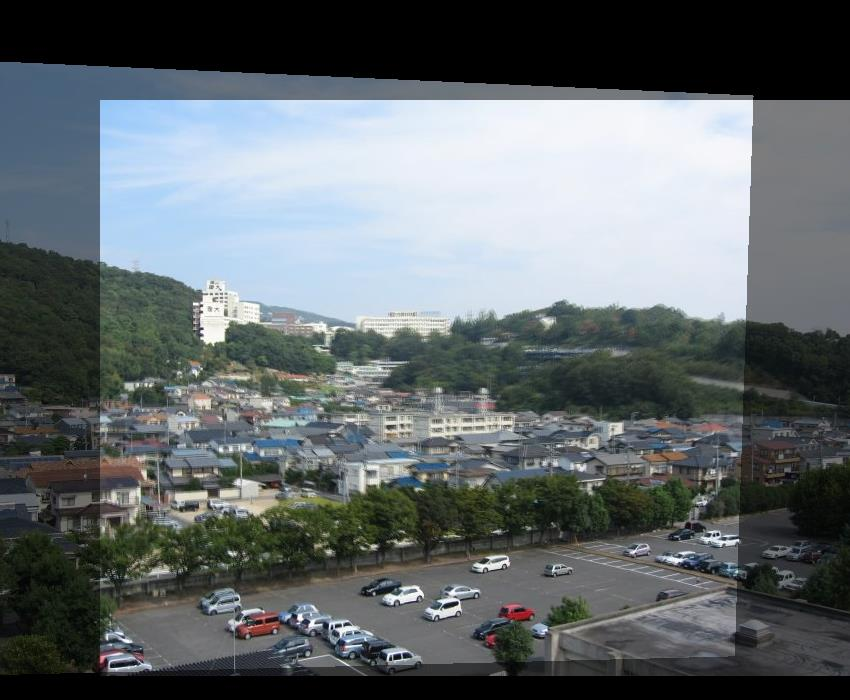
\includegraphics[scale=.6]{./img/out.jpg}

\section{並列化}

openMPによる並列化によって,calcSSDtable関数の処理時間を0.771msecから
0.349msecへ短縮した.

\begin{lstlisting}
void calcSSDtable(Matrix* mt,
    Image* im, int x1[][2], int N1,
    Image* im2, int x2[][2], int N2) {
    int i, j;
#pragma omp parallel for private (j)
    for (i = 0; i < N1; i++)
        for (j = 0; j < N2; j++)
            Elem(mt, i, j) = ImageSSD(im, x1[i][0], x1[i][1],
                im2, x2[j][0], x2[j][1]);
}
\end{lstlisting}

\section{考察}

今回の実験では,各画像から得られた特徴点群の対応付けを行う処理を記述した.
貪欲法を2つの方法で実装したが,方法1と2で異なる結果が得られた.
確認ページ\url{https://moodle.el.okayama-u.ac.jp/pluginfile.php/973944/mod_resource/content/43/matchViewer.html}
にて,得られた特徴点座標の組を入力すると,方法1で得た座標組が正しくないことが分かった.

方法1で間違った結果になった原因は,第1画像の特徴点らしさの高い点の対になる特徴点を
探すやり方だったからである.
第1画像の特徴点iに対しての類似度が一番高い第2画像の特徴点jだったとして,
特徴点jに対しての類似度が高い点がほかにあるかもしれないからである.

方法2では,特徴点の組すべてから類似度の高い組を選んでいたので,
間違いが少ないのだと考える.



\end{document}